\setcounter{page}{1}

\section{Introduction} % (fold)
\label{sec:introduction}

This the final report for a project in the course ``Fault tolerant systems'' 02228. The purpose of this report is to document our experience implementing a consensus algorithm i.e. Raft. Our approach to this is to take the basic description of Raft and iteratively construct a test for each behaviour the algorithm should have and implement its functionality that satisfies the given test.\\

The fundamental problem, when talking about consensus in a distributed system, will be presented at start. This will then show the motivation behind the project itself. And, as many solutions to this problem already exists, it should also be discussed why Raft in particular is relevant in the context of this project.

\subsection{Problem}
Reaching consensus in a distributed system means that all or at least the majority of processes in the network agree on some value or state of the entire system. This is often needed when processes might be faulty thus bringing reliability and availability at stake on single-point-of-failure. Upholding these properties in a given distributed system then relies on the architecture utilised and hardware implemented in the processes.\\ A simple solution to this could be to initiate a vote among all correct processes on to what the value is, in which the value is the result of the majority vote. The figure \ref{consensus} below illustrates an example of a distributed system consisting of a number of notes. The value \textit{x} is what the system must agree upon. Though here we have faulty process \textit{P1}, which is responsible to give back the result. Taking the fact of connectivity of system aside, the system will become unavailable because of the now faulty process. \\

% What is 'this' in ... the system will suffer from this...

% changed to 'will become unavailable'

\begin{figure}[h]
	\centering
	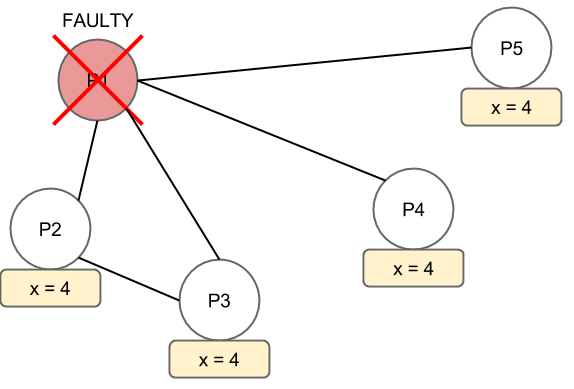
\includegraphics[width=0.5\textwidth]{consensus}
	\caption{A distributed system consisting of a number of nodes with a faulty one.}
	\label{consensus}
\end{figure}

The fundamental problem behind this, is that you cannot rely on the individual processes to be reliable and thus solely store the value. This means, that every process should store this value and should be able to be altered somehow. This boils down to a well-known problem - The Two Generals Problem.

% Måske burde the two generals problem komme her?

% Enig, har sat det ind her i stedet for.

\subsection{Motivation}
The elements of the problem presented serve as motivation behind consensus in a system of unreliable components. Because how do you know for certain what a value is, when you for sure know that some components must be faulty at some point?

\subsubsection{The Two Generals Problem}
The basic problem of reaching consensus in a distributed network can be illustrated by the Two Generals Problem analogy.

\begin{figure}[h]
	\centering
	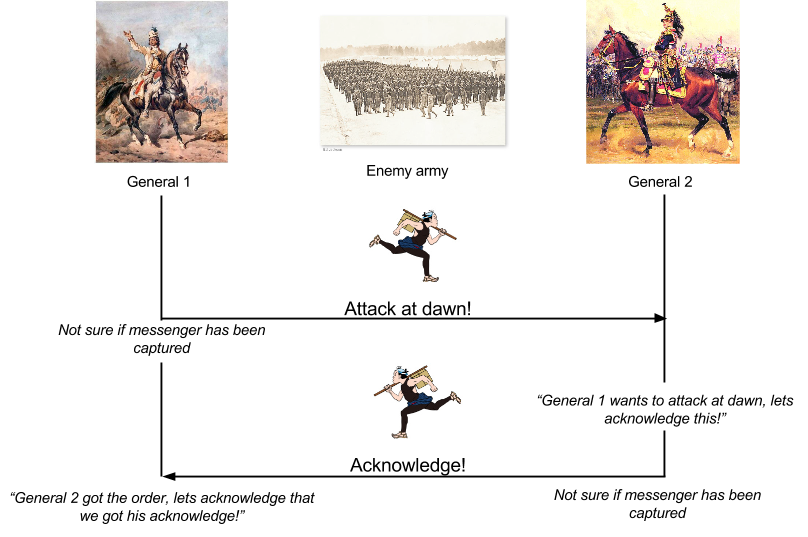
\includegraphics[width=0.8\textwidth]{twogenerals}
	\caption{Two generals tries to agree on when to attack the enemy by sending a messenger, but they are not sure the messenger survives his trip between their camps.}
	\label{generals}
\end{figure}

In the figure\ref{generals} below we see two generals of the same army who want to attack an enemy army. But they have to attack at the same time in order to win. They cannot communicate directly to each other since they are at different fronts of the battlefield i.e. in their own camps. In the context of a distributed system, the generals here can be seen as two processes trying to agree on a value.
General 1 then sends out a messenger to tell the second general, that they should attack at dawn. The second general then receives this message, but the first general cannot be sure of this (the messenger might be captured or killed by the enemy on his way to the second general and vice versa). Again, in the context of distributed system, the unreliability of messenger can directly related back to the unreliability of message transmission in a normal distributed system. In terms of Byzantine failure, this can be illustrated by the messenger being captured by the enemy and turned to spy on the generals i.e. given false information.
So the second general sends the messenger back in order to acknowledge this. But the first general also has to acknowledge this, resulting in a never ending run for the poor messenger - thus the generals can never agree on when to attack the enemy.

\subsubsection{Properties of distributed consensus}
When want to define consensus, the goal is to satisfy a set of requirements i.e. properties that the distributed system must uphold. These are used to describe the systems fault tolerant features related to faulty processes. A faulty process can either fail by crashing or experience a Byzantine failure. Such a failure in the context of distributes system occur when e.g. a process for some reason transmits incorrect or malicious data throughout the network. Due to the arbitrary results of these kinds of failures, properties of a system are often distinguished by either tolerating them or not. A main difference in terms of properties of a system whether it tolerates Byzantine failures or not, is the validity and integrity. The integrity property for a system that does not tolerate Byzantine failures is as following\cite{DistributedSystems}.

\begin{itemize}
\item non-Byzantine failure tolerant:
	\begin{itemize}
	\item \textbf{Validity}: If all processes propose the same value \textit{v}, then all correct processes decide \textit{v}.
	\item \textbf{Integrity}: Every correct process decides at most one value, and if it decides some value \textit{v}, then \textit{v} must have been proposed by some process.
	\end{itemize}
\item Byzantine failure tolerant:
	\begin{itemize}
	\item \textbf{Validity}: If all correct processes propose the same value \textit{v}, then all correct processes decide \textit{v}.
	\item \textbf{Integrity}: If a correct process decides \textit{v}, then \textit{v} must have been proposed by some correct process.
	\end{itemize}
\end{itemize}

The clearest commonality here, is that you should always be able to say that all correct processes must be able to decide on the same value or state, as mentioned earlier. Though the main difference is that with Byzantine processes, you must be able to say if they are all correct before stating they can derive the same value. This fact differentiates many solutions to this problem, depending on which property set they can satisfy. \\
Also, as discussed in \cite{Raft} a consensus algorithm for a non-Byzantine system has the following properties: safety, availability, timing interdependency, and majority vote on procedure calls. The safety property can be directly related back to our validity and integrity properties, as the system's safety and availability is measured be the correctness of return result upon a request.

% section introduction (end)
